\documentclass[]{article}\usepackage[]{graphicx}\usepackage[]{color}
%% maxwidth is the original width if it is less than linewidth
%% otherwise use linewidth (to make sure the graphics do not exceed the margin)
\makeatletter
\def\maxwidth{ %
  \ifdim\Gin@nat@width>\linewidth
    \linewidth
  \else
    \Gin@nat@width
  \fi
}
\makeatother

\definecolor{fgcolor}{rgb}{0.345, 0.345, 0.345}
\newcommand{\hlnum}[1]{\textcolor[rgb]{0.686,0.059,0.569}{#1}}%
\newcommand{\hlstr}[1]{\textcolor[rgb]{0.192,0.494,0.8}{#1}}%
\newcommand{\hlcom}[1]{\textcolor[rgb]{0.678,0.584,0.686}{\textit{#1}}}%
\newcommand{\hlopt}[1]{\textcolor[rgb]{0,0,0}{#1}}%
\newcommand{\hlstd}[1]{\textcolor[rgb]{0.345,0.345,0.345}{#1}}%
\newcommand{\hlkwa}[1]{\textcolor[rgb]{0.161,0.373,0.58}{\textbf{#1}}}%
\newcommand{\hlkwb}[1]{\textcolor[rgb]{0.69,0.353,0.396}{#1}}%
\newcommand{\hlkwc}[1]{\textcolor[rgb]{0.333,0.667,0.333}{#1}}%
\newcommand{\hlkwd}[1]{\textcolor[rgb]{0.737,0.353,0.396}{\textbf{#1}}}%

\usepackage{framed}
\makeatletter
\newenvironment{kframe}{%
 \def\at@end@of@kframe{}%
 \ifinner\ifhmode%
  \def\at@end@of@kframe{\end{minipage}}%
  \begin{minipage}{\columnwidth}%
 \fi\fi%
 \def\FrameCommand##1{\hskip\@totalleftmargin \hskip-\fboxsep
 \colorbox{shadecolor}{##1}\hskip-\fboxsep
     % There is no \\@totalrightmargin, so:
     \hskip-\linewidth \hskip-\@totalleftmargin \hskip\columnwidth}%
 \MakeFramed {\advance\hsize-\width
   \@totalleftmargin\z@ \linewidth\hsize
   \@setminipage}}%
 {\par\unskip\endMakeFramed%
 \at@end@of@kframe}
\makeatother

\definecolor{shadecolor}{rgb}{.97, .97, .97}
\definecolor{messagecolor}{rgb}{0, 0, 0}
\definecolor{warningcolor}{rgb}{1, 0, 1}
\definecolor{errorcolor}{rgb}{1, 0, 0}
\newenvironment{knitrout}{}{} % an empty environment to be redefined in TeX

\usepackage{alltt}
\usepackage{fontspec}
\usepackage{graphicx}
\usepackage{float}
\usepackage[hidelinks]{hyperref} % For linking Github

\usepackage[left=1.27cm, top=1.27cm, right=1.27cm, bottom=2.54cm]{geometry}

\usepackage{pbox}
\setmainfont[Scale=1]{Cambria}
\linespread{1.25}
\usepackage{pdflscape}

\usepackage{setspace}
\usepackage[document]{ragged2e} % For left-alignment.
\usepackage{parskip} % For space between paragraphs
% For the big table in the Appendix.
\usepackage{longtable}
\usepackage[small,bf,singlelinecheck=off]{caption}

% If you use Biber, then you will have to compile and recompile.
% But Biber seems to be the preferred choice.
\usepackage[backend=biber,sorting=none,style=numeric-comp]{biblatex}

\addbibresource{tmle.bib} % Critical that you put .bib in here!
\IfFileExists{upquote.sty}{\usepackage{upquote}}{}
\begin{document}
\title{Hospital readmissions and targeted maximum likelihood estimation}
\author{Aman Verma}
\date{\today}

\begin{abstract}







Background: Hoping to improving quality of hospital care, the US and other jurisdictions financially penalize hospitals with poor (confounder-adjusted) 30-day readmission rates. Although hospital administrative data are information-rich, confounder adjustment tends to be crude. Non-parametric machine learning techniques can take advantage of these rich data to predict readmission, but cannot isolate the independent effect of hospitals on readmission risk.

Research Design: To estimate the effect of care at different hospitals on 30-day readmission risk, we used targeted maximum likelihood estimation (TMLE), which allowed us to use a non-parametric machine learning technique (random forest) to take advantage of the rich confounder data. We used an 11-year cohort of 65-year-old patients from 20 hospitals in Montreal, Canada, and developed three models to estimate the marginal readmission risk at each of the hospitals after hospitalization for heart failure, acute myocardial infarction (AMI), and pneumonia. We controlled for hundreds of confounders including outpatient drug prescriptions, medical procedures, and diagnoses. We compared the TMLE-estimated risk to a logistic regression model that only crudely adjusted for confounding.

Results: Within each hospital, crude readmission risk varied widely across the twenty hospitals for AMI 2,525 / 15,746 (16\%), heart failure 5,520 / 24,847 (22\%), and pneumonia 3,183 / 20,421 (16\%). When crudely controlling for confounding, and compared to an arbitrary reference hospital, the odds ratio ranged from 0.95-1.02 for AMI, 0.92-1.04 for heart failure, and 0.96-1.04 for pneumonia. When we applied TMLE,
the odds ratio ranged from 0.57-2.30 for AMI, 0.50-1.85 for heart failure, and 0.47-1.55 for pneumonia.

Conclusion: Our results suggest that crudely adjusted hospital readmission rates will underestimate the differences between hospitals. Using TMLE, we could take advantage of rich confounder data, and reveal wide differences in quality of care between hospitals.

\end{abstract}

\section{Introduction}
% Work this in:
% To measure quality of care, administrators have selected three common admission reasons with high readmission risk: acute myocardial infarction (AMI), pneumonia, and heart failure.\supercite{us_government_public_2012}
In the US and other jurisdictions, administrators have sought to improve quality of care by financially penalizing hospitals with poor readmission rates.\supercite{institute_of_medicine_u.s.._division_of_health_care_services_medicare_1990} To avoid penalizing high quality of care at hospitals that admit sicker (more likely to be readmitted) patients, readmission rates are adjusted for patient-level confounding.\supercite{us_government_public_2012} Although hospital readmission rates are typically only adjusted for a few well-known confounders such as age, sex, previous readmissions, and summarized comorbidity scores,\supercite{kansagara_risk_2011} healthcare administrative data are often information-rich, including drug prescriptions, diagnoses, and medical procedures.

% Maybe give some clue as to why they aren't being used?
Some epidemiologists have argued for the application of machine learning techniques to handle newly available information-rich data sources.\supercite{glymour_invited_2013} Non-parametric machine learning techniques can accurately discriminate patient readmission risk using hundreds of variables in a computationally efficient way.\supercite{friedman_regularization_2010} Non-parametric models also allow us to avoid specifying a functional form, making it easier to detect complex relationships like multi-way interactions. However, most machine learning techniques were developed for prediction rather than inference; we cannot use them alone to isolate (target) effects measures of specific variables, such as care at a particular hospital, on readmission risk.

% Instead of summarizing comorbidity scores using expert knowledge, we use the data to develop a comorbidity score specific to the problem at hand.
The targeted maximum likelihood estimator (TMLE), is a doubly-robust technique that uses propensity scores to estimate target parameters of interest, and allows the incorporation of machine learning techniques.\supercite{van_der_laan_targeted_2011}  In TMLE, two (possibly non-parametric) two models are developed: one to estimate the probability of exposure (the propensity score), and another model to estimate the probability of the outcome. These two probabilities are combined in a parametric model with only the parameter of interest. In this way, the discriminative power of non-parametric models can be used to extract estimates of parameters of interest.

% What is the study question?
Although some studies have used the rich confounder data in combination with machine learning techniques to predict hospital readmissions\supercite{he_mining_2014, hosseinzadeh_assessing_2013}, no study to our knowledge has used these data to draw causal inference on the effect of quality of care on readmissions. In this study, we sought to estimate the independent effect of hospital care on the 30-day readmission for twenty Montreal hospitals, within three different admission diagnoses (pneumonia, heart failure, and acute myocardial infarction). We used a non-parametric machine learning technique, (random forest\supercite{breiman_random_2001}), with TMLE to take advantage of the rich confounder data and minimize bias in our estimate of readmission risk.

\section{Methods}

\subsection{Study Design}
% Cohort selection
We used a cohort extracted from a Canadian provincial (Quebec) administrative database of hospitalizations, obtained from the \emph{Régie de l'assurance maladie du Québec} (RAMQ). We enrolled patients into this cohort on the month that two conditions were satisfied: 1) they had at least one diagnosis of a respiratory illness (the exact list of respiratory International Classification of Diseases, 9th Revision [ICD-9] codes is given in Table \ref{icd_codes} the Appendix) between January 1st, 1996 and March 31, 2006 (the study period), while living in the 2006 census metropolitan area of Montreal, and 2) were at least 65 years of age. We used this cohort because it contains the majority of 65-year-old patients who were hospitalized in the region during the study period.

From among this cohort, we selected hospital discharges for those who had accrued at least one continuous year in the cohort preceding the day of admission. We restricted our data to only the discharges from the twenty hospitals with the most discharges of patients 65 years of age or older within the study period; the twenty hospitals accounted for 75\% of all such discharges.  We only selected hospital discharges which resulted from hospital stays of at least one day. Therefore, the earliest possible hospital discharge was January 2, 1997.

% Disease types
From among the identified hospital discharges, we selected only those with one of three high-volume admission diagnoses with high rates of hospital readmissions: pneumonia, acute myocardial infarction (AMI), and heart failure. We identified each of the admission diagnoses using ICD-9 codes; for pneumonia we used codes ranging from 480-487, for heart failure we used all 428 codes, and for AMI we used all 410 codes. The following methods were applied individually to all three disease subsets.

\subsection{Hospital readmissions}
The unit of analysis was the hospital discharge; a person could be discharged multiple times. A hospital readmission was defined as an emergency hospital admission to any Quebec hospital in the 30 days following a discharge.  A person who died or had a non-emergency readmission in the 30 days following discharge was considered not readmitted.

\subsection{Confounders and Risk Factors}
% The basic demographics and time-related confounders.
For each hospital discharge, we collected plausible confounders that measured states at the time of, or prior to, admission. We used the demographic characteristics (age at time of admission (years), sex, birth year-month), the number of previous readmissions (within the preceding year), the admission diagnosis (as measured by the specific ICD-9 code). We also included the day of week of discharge, which has been previously shown to have an association with readmissions\supercite{van_walraven_risk_2002}, and the month of discharge, because we hypothesized that readmission risk would vary by season in Montreal.

% Procedures, drugs, and diagnoses.
Additionally, for each discharge, we collected the Quebec hospital diagnoses, Quebec hospital procedures, and drugs dispensed outside of the hospital but inside Quebec, in the year preceding the admission. The hospital procedures were recorded in the Canadian Classification of Diagnostic, Therapeutic, and Surgical Procedures (CCP) system. Hospital diagnostic codes were coded using the ICD-9 system. Finally, drugs which were prescribed and dispensed outside the hospital, and were being taken on the day of admission were also recorded for each patient in the \emph{code commune} system, which categorizes drugs based on the chemical compound. To ease computation, before fitting any model, we removed any diagnosis, procedure or drug that occurred less than 30 times among all discharges. We chose 30 because it appeared to be a natural breakpoint; if the number of variables included is a function $f$ of the threshold, then the first derivative of $f$ dropped at 30 for all three disease categories.

% Area of residence.
We believed that residential location would strongly affect the probability of admission to the hospital nearest that census tract. We included it in our models because we also expected it to crudely approximate a (expected) confounder: socio-economic status.  We used the residential postal code at the time of admission to assign each patient in the cohort to a census tract, as defined by the 2006 Canadian census. (Census tracts contain between 2,500 and 8,000 people, and, at the time of their creation, are demarcated so as to maximize homogeneity of socioeconomic characteristics.)\supercite{statistics_canada_2006_2007}

\subsection{Statistical Analyses}
For each discharge $i$, we sought to estimate the effect of each of the twenty hospitals $A \in \left\{ {a_1, \dots ,a_{20}}\right\}$ on 30-day readmission ($Y$), accounting for the vector of confounders ($W$). To estimate this risk, we used targeted maximum likelihood estimation, which consisted of several steps. We first estimated of a model of the propensity score $g=Pr(A|W)$ (using random forest described below). Next, we estimated of a model of readmission risk based on the confounders $W$ and the variables for each of the hospitals $Q=Pr(Y=1|A,W)$. We then calculated $h_a(A,W)$ (sometimes referred to as the clever covariate) described in equation \ref{logistic_clever_covariate}

\begin{equation}
\label{logistic_clever_covariate}
h_a(A,W)=\frac{I(A=a)}{g(a|W)}
\end{equation}

(where $I$ is the indicator function which evaluates to 1 when its argument is true, and 0 otherwise), and solved for all ${\epsilon}_a$ in fluctuation function described in equation \ref{logistic_fluctuation_function}.

\begin{equation}
\label{logistic_fluctuation_function}
Y_i=expit(logit(Q(Y_i|A_i,W_i)) + \sum_{j=1}^{20} {\epsilon}_{a_j} \times h_{a_j}(A_i,W_i))
\end{equation}

We solved for all twenty ${\epsilon}_a$ by regressing the 30-day readmission outcome $Y$ (with a logit link function) onto $h_a(A,W_i)$ (with no intercept) offset by the inverse logit of the initial estimate of readmission risk $Q=(Y|A,W)$. Finally, for each discharge, we computed the estimated risk of 30-day readmission for all twenty counterfactual conditions (the risk of readmission for every discharge as if they had attended different hospital) using Equation \ref{Q_star_logistic}.

\begin{equation}
\label{Q_star_logistic}
Q^*_{ai}= expit(logit(Q(Y|a,W_i)) + \frac{\epsilon}{g(a|W)})
\end{equation}

For each hospital, we then calculated the mean readmission risk ($Q^*_a$) and associated odds ratio.

% Random forest
To estimate both models $g(A_i|W_i)$ and $Q(Y_i|A,W_i)$, we used a random forest, a non-parametric model based on decision trees.\supercite{breiman_random_2001} Decision trees use the independent variables ($W_i$) to repeatedly split data into partitions that are as homogeneous as possible with respect to the outcome of interest (specifically measured with the Gini coefficient\supercite{gini_variabilita_1912}). Random forest improves decision trees by using bootstrap aggregation (bagging); multiple decision trees are grown on bootstrap replicates (sampled with replacement) to avoid overfitting. Additionally, within each tree, only a sample of the covariates is used (in our case we used a square root of the number of variables included in the mode, rounded down).

For both models $g(A_i|W_i)$ and $Q(Y_i|A,W_i)$, we arbitrarily chose to grow 1200 trees, and then measured the accuracy as a function of the number of trees to ensure that growing further trees would be unlikely to improve accuracy. Because the model was used solely to estimate the \emph{probability} of admission to to specific hospitals (and not to predict exactly which hospital was attended), when calculating the Gini coefficient to build the trees we configured the model to favor calibration over discrimination: we weighted each of the twenty predicted hospitals by the inverse of the proportion of discharges at that hospital. When measuring the accuracy for each discharge, we only used trees for which the discharge was "out-of-bag", that is, we only used trees for which the bootstrap sample did not include the discharge.

% Variable importance
To describe importance of the covariates in both models $g(A_i|W_i)$ and $Q(Y_i|A,W_i)$, for each variable, we measured the decrease in the Gini coefficient for each partition in which the variable was used, in every tree. A low Gini (i.e. higher decrease in Gini) means that a particular predictor variable plays a greater role in partitioning the data into the defined classes. We plotted the densities of variables with four different classes (census tract, procedure, diagnosis and drug) at different levels of Gini decreases.

% Calibration
Random forest classifies each item by majority vote: each tree in the forest assigns each discharge to a specific class. Although the vote proportion is between zero and one, it is not calibrated well as a probability. To calibrate the vote proportion, we used Platt scaling\supercite{platt_probabilistic_1999} (logistic regression of the outcome ($Y_i$) on to the vote proportion).

% gbound
When the probability of exposure $g(A|W)$ is very low, that discharge would receive a large weight in estimating $Q^*$. For any $g(A|W)$ below some fixed value $\delta$, we set $g(A|W)$ to $\delta$. We recomputed our analyses at 31 different values of $\delta$, ranging from $10^{-2}$ to $10^{-5}$, decreasing the exponent at intervals of 0.1.

% Comparison to assessment with comorbidity scores
Finally, we compared our results of our analysis with a logistic regression for 30-day readmission. In this model, we included only the age, sex, number of previous admissions, and the Charlson comorbidity score (Elixhauser version)\supercite{elixhauser_comorbidity_1998}, along with indicator variables representing the hospitals themselves.

\subsection{Software}
The data were cleaned and prepared for statistical analysis using the Postgres relational database (version 9.3.5). We implemented our models using the R statistical package (version 3.1.1),\supercite{team_r:_2014} using the "bigrf" package (version 0.1.11) to grow the random forests.\supercite{lim_bigrf:_2014} We plotted our figures using the "ggplot2" package (version 1.0.0) .\supercite{wickham_ggplot2:_2009} All the code to develop used to process our data, fit our models, and typeset this article is \href{https://github.com/nograpes/tmle_readmissions}{available for download at Github}.

\section{Results}


Over the course of January 2, 1996 to March 31, 2006, 482,064 people were entered into our cohort. Among these, 16,521 were ever admitted for pneumonia, 13,884 were ever admitted for AMI, and 15,822 were ever admitted for heart failure. People ever admitted for pneumonia had a mean (median) 1.2 (1) pneumonia admissions, heart failure patients had a mean (median) 1.6 (1) heart failure admissions, and AMI patients had a mean (median) 1.1 (1) AMI admissions. In total, we analyzed 20,421 pneumonia discharges, 15,746 AMI discharges, and 24,847 heart failure discharges.

% The accuracy of random forest.
% The types of variables that were important for both g and Q.
The accuracy of the random forest (for both models $g$ and $Q$) did not appear to improve significantly beyond 125 trees (see Figure \ref{fig:error_rate_for_g_and_Q} in the appendix). In Figure \ref{fig:variable_importance_by_model_and_class} we plot the importance of variables (as measured by the Gini coefficient) in the random forest models for four variable classes, for all disease subsets for both the $g$ and $Q$ model. Although census tracts were found to be important in prediction of hospital choice,  the other three variable classes were had a high density of important variables as well. The prescription drugs in particular had a high proportion of important variables, and generally the lowest proportion of unimportant variables. For the $Q$ model, the variable density appeared bimodal within variable importance for all four variable classes. Additionally, the pre-admission drug prescriptions appeared to be strongly important in predicting readmission for all pneumonia, heart failure, and AMI admissions.

% The distribution of g
The predicted probability of admission to any particular hospital ($g=Pr(A=a|W)$) was less than 5\% in 88\% of cases (across all disease subsets and hospitals).  We set $\delta$ (the lower bound of $g$ when used to fit the $\epsilon$ values for $Q^*$), to two different values, $10^{-2}$ and $10^{-2.5}$. Across all disease subsets and hospitals, 39\% of discharge/hospital combinations and a $g$ less than $10^{-2}$, and 4\% had a $g$ less than $10^{-2.5}$. Figure \ref{fig:dist_g_zoomed} (in the Appendix) describes the histogram of $g$ when it is below 0.05 for each disease/hospital combination separately.

% The tables
% The in hospital death rates
% The crude model.
% The TMLE models.
The unadjusted proportion of patients readmitted in 30 days varied across hospitals for each disease subset (Tables 1-3). The linear correlation between the proportion of deaths during hospital stay and the proportion readmitted was (0.19, \ensuremath{-0.55}, \ensuremath{-0.28}) among AMI, heart failure, and pneumonia admissions respectively. Using a model that adjusts for a few well-known confounders, for AMI, heart failure, and pneumonia respectively, one, three, and five hospitals had significantly different odds than the reference hospital. Notably, the significant odds ratios are all relatively small, with point estimates ranging from 0.92 - 1.04. In contrast, in the TMLE models, at both values of $\delta$, for all admission diagnoses, nearly all of the hospitals had significantly different odds than the reference hospital.

% Effect of delta
In some hospitals and disease subsets, the parameter $\delta$, (the lower bound on the probability of exposure $g(A|W)$) had a considerable effect on the marginal risk and the associated odds ratios. For example, for AMI (shown in Table 1), the marginal risk for hospital 17 increases by six percent when $\delta$ decreases from $10^{-2}$ to $10^{-2.5}$. In Figure \ref{fig:effect_of_gbound}, we display the marginal risk for each of the twenty hospitals and disease subsets as a function of the parameter $\delta$. For many hospitals, the effect was quite strong; for pneumonia admissions, hospital 16 went from having the second-lowest marginal risk when $\delta=0.1$ to having the highest marginal risk when $\delta=0.025$.


% Variable importance.
\begin{figure}[H]
    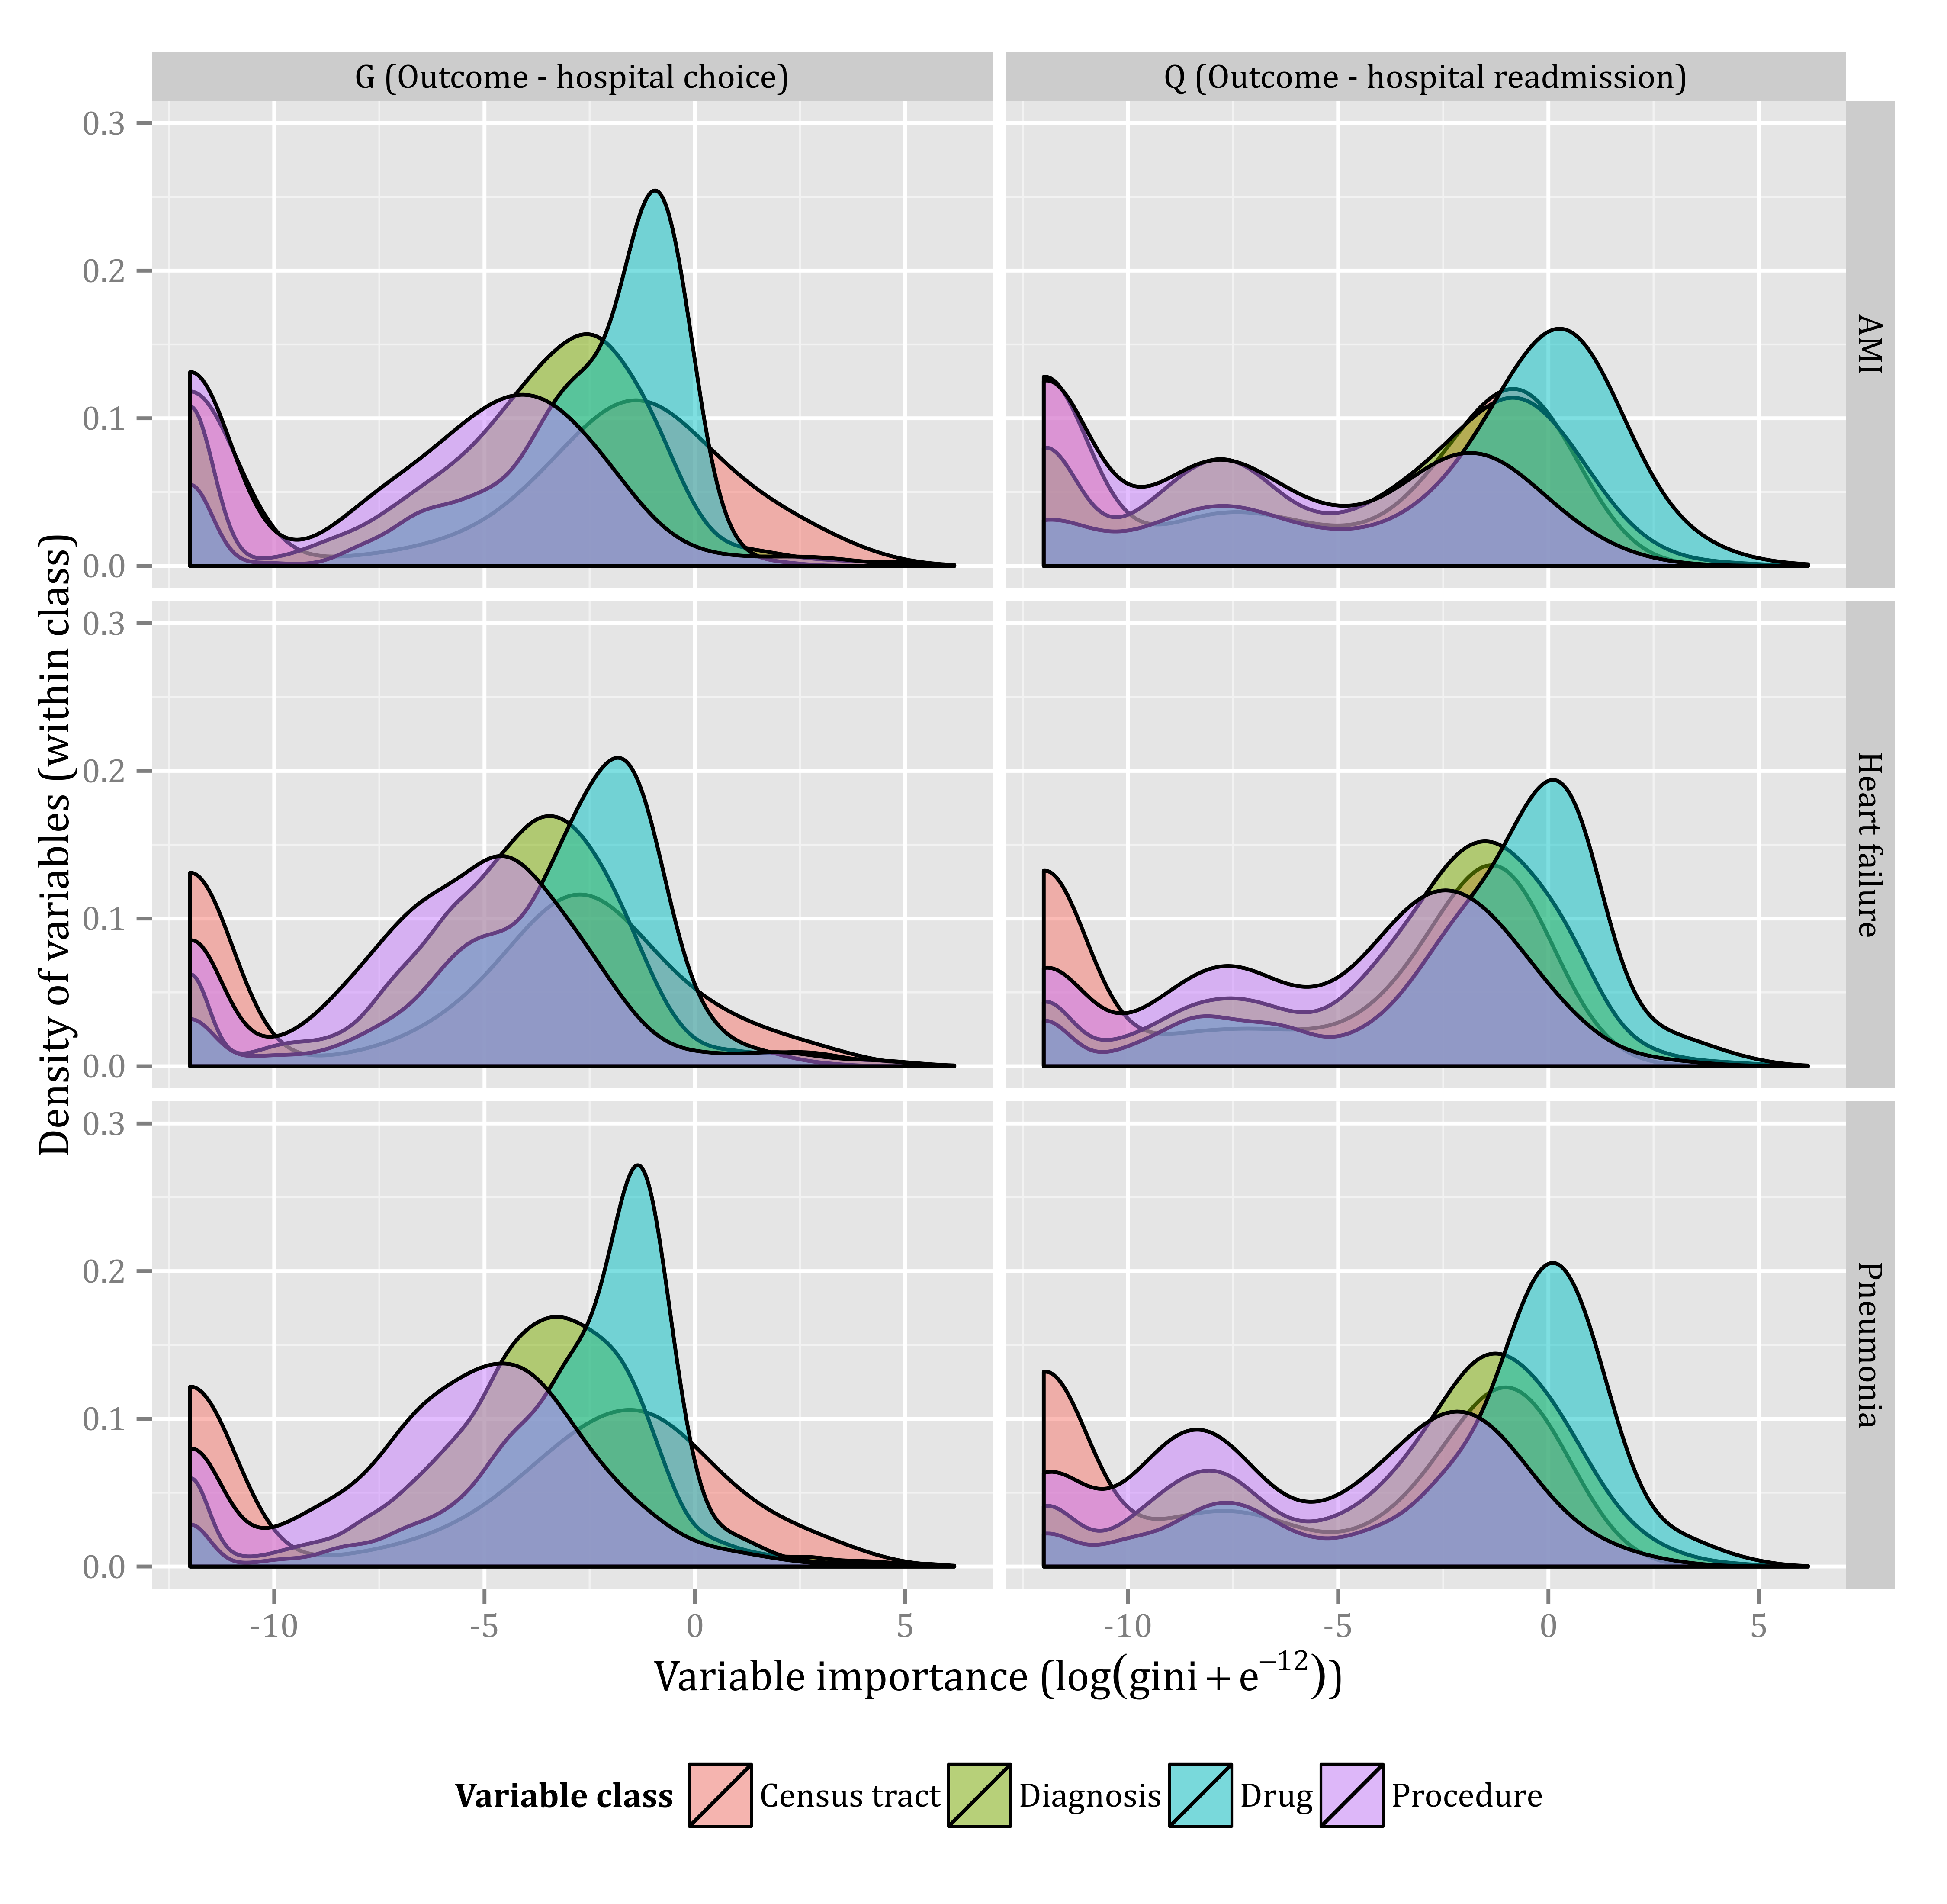
\includegraphics{../figures/variable_importance_by_model_and_class.png}
    \caption[Error rate for random forest model of hospital choice.]
{Variable importance by model and variable class. For each random forest classifier, the variable importance was measured by the decrease in the Gini coefficient when that variable splits a node. The horizontal axis within each panel is displayed on a $log_e$ scale. Some variables had exactly zero importance; to avoid evaluating the logarithm of zero, we added a small constant ($e^{-12}$) to the measure of variable importance. The vertical axis in each panel represents the variable density at the corresponding level of variable importance. To transform the individual variable importances into a continuous density, we smoothed using a Gaussian kernel density estimator, using Silverman's 'rule-of-thumb' \supercite{silverman_density_1986} to select the bandwidth. The density is measured separately for each class; the area under each variable class curve is exactly one.
}
   \label{fig:variable_importance_by_model_and_class}
\end{figure}

% Table code.
\begin{landscape}
\setmainfont[Scale=1]{Cambria}
\linespread{1}
%latex.default(pre.format, file = "", col.just = rep("r", 10),     cgroup = c("", "Logistic regression", tmle.colnames), n.cgroup = c(4,         2, rep(2, length(tmle.colnames))), rowlabel = "Hsp.",     caption.loc = "bottom", caption = paste("Risk of 30-day readmission after admission for ",         pretty_names_lower[disease], " in twenty Montreal hospitals. ",         ifelse(disease == diseases[1], caption.text, caption.text.see.other.table)),     label = paste(disease, "table", sep = "_"))%
\begin{table}[!tbp]
\begin{center}
\begin{tabular}{lrrrrcrrcrrcrr}
\hline\hline
\multicolumn{1}{l}{\bfseries Hsp.}&\multicolumn{4}{c}{\bfseries }&\multicolumn{1}{c}{\bfseries }&\multicolumn{2}{c}{\bfseries Logistic regression}&\multicolumn{1}{c}{\bfseries }&\multicolumn{2}{c}{\bfseries TMLE ($\delta=10^{-2}$)}&\multicolumn{1}{c}{\bfseries }&\multicolumn{2}{c}{\bfseries TMLE ($\delta=10^{-2.5}$)}\tabularnewline
\cline{7-8} \cline{10-11} \cline{13-14}
\multicolumn{1}{l}{}&\multicolumn{1}{c}{Admitted}&\multicolumn{1}{c}{Died}&\multicolumn{1}{c}{Discharged}&\multicolumn{1}{c}{Readmitted}&\multicolumn{1}{c}{}&\multicolumn{1}{c}{Odds ratio}&\multicolumn{1}{c}{Marginal}&\multicolumn{1}{c}{}&\multicolumn{1}{c}{Odds ratio}&\multicolumn{1}{c}{Marginal}&\multicolumn{1}{c}{}&\multicolumn{1}{c}{Odds ratio}&\multicolumn{1}{c}{Marginal}\tabularnewline
&&\multicolumn{1}{c}{{\scriptsize (\%)}}&&\multicolumn{1}{c}{{\scriptsize (\%)}}&&\multicolumn{1}{c}{{\scriptsize (95\% CI)}}&\multicolumn{1}{c}{{\scriptsize risk}}&&\multicolumn{1}{c}{{\scriptsize (95\% CI)}}&\multicolumn{1}{c}{{\scriptsize risk}}&&\multicolumn{1}{c}{{\scriptsize (95\% CI)}}&\multicolumn{1}{c}{{\scriptsize risk}}\tabularnewline
\hline
1&$ 763$&112 (15)&$ 651$&105 (16)&&0.98 (0.95-1.01)&$0.16$&&0.86 (0.83-0.89)&$0.16$&&0.77 (0.74-0.81)&$0.14$\tabularnewline
2&$1557$&148 (10)&$1409$&191 (14)&&0.97 (0.95-1.00)&$0.15$&&0.85 (0.82-0.87)&$0.15$&&0.85 (0.82-0.87)&$0.15$\tabularnewline
3&$ 606$&83 (14)&$ 523$&84 (16)&&0.98 (0.95-1.02)&$0.16$&&1.01 (0.97-1.05)&$0.18$&&1.09 (1.04-1.14)&$0.19$\tabularnewline
4&$1022$&125 (12)&$ 897$&136 (15)&&0.97 (0.94-1.00)&$0.15$&&0.72 (0.69-0.74)&$0.13$&&0.72 (0.69-0.74)&$0.13$\tabularnewline
5&$ 729$&150 (21)&$ 579$&98 (17)&&0.98 (0.95-1.02)&$0.16$&&0.75 (0.72-0.77)&$0.14$&&0.73 (0.71-0.76)&$0.14$\tabularnewline
6&$ 826$&119 (14)&$ 707$&106 (15)&&0.98 (0.94-1.01)&$0.15$&&0.57 (0.54-0.60)&$0.11$&&0.57 (0.54-0.60)&$0.11$\tabularnewline
7&$1491$&241 (16)&$1250$&216 (17)&&0.99 (0.96-1.01)&$0.16$&&1.04 (1.01-1.06)&$0.18$&&1.03 (1.01-1.06)&$0.18$\tabularnewline
8&$1270$&198 (16)&$1072$&138 (13)&&0.95 (0.92-0.98)&$0.13$&&0.69 (0.67-0.71)&$0.13$&&0.69 (0.67-0.71)&$0.13$\tabularnewline
9&$ 780$&152 (19)&$ 628$&130 (21)&&1.01 (0.97-1.05)&$0.19$&&0.54 (0.51-0.56)&$0.10$&&0.52 (0.50-0.54)&$0.10$\tabularnewline
10&$ 778$&124 (16)&$ 654$&123 (19)&&1.01 (0.97-1.05)&$0.19$&&1.19 (1.15-1.23)&$0.20$&&1.27 (1.22-1.31)&$0.21$\tabularnewline
11&$ 705$&125 (18)&$ 580$&97 (17)&&0.99 (0.96-1.03)&$0.17$&&0.89 (0.85-0.92)&$0.16$&&0.90 (0.86-0.94)&$0.16$\tabularnewline
12&$1284$&266 (21)&$1018$&166 (16)&&0.99 (0.96-1.02)&$0.16$&&0.90 (0.88-0.93)&$0.16$&&0.90 (0.88-0.93)&$0.16$\tabularnewline
13&$ 739$&86 (12)&$ 653$&110 (17)&&0.99 (0.95-1.02)&$0.16$&&1.19 (1.16-1.23)&$0.20$&&1.22 (1.18-1.27)&$0.21$\tabularnewline
14&$1307$&184 (14)&$1123$&210 (19)&&(Reference)&$0.18$&&(Reference)&$0.18$&&(Reference)&$0.18$\tabularnewline
15&$1152$&168 (15)&$ 984$&129 (13)&&0.97 (0.95-1.01)&$0.15$&&0.70 (0.68-0.73)&$0.13$&&0.70 (0.68-0.73)&$0.13$\tabularnewline
16&$ 408$&70 (17)&$ 338$&43 (13)&&0.97 (0.93-1.01)&$0.15$&&0.84 (0.80-0.88)&$0.15$&&0.84 (0.80-0.89)&$0.15$\tabularnewline
17&$ 807$&123 (15)&$ 684$&134 (20)&&1.02 (0.99-1.06)&$0.20$&&1.76 (1.72-1.81)&$0.27$&&2.30 (2.23-2.37)&$0.33$\tabularnewline
18&$ 894$&144 (16)&$ 750$&116 (15)&&0.98 (0.95-1.01)&$0.16$&&0.91 (0.87-0.94)&$0.16$&&0.91 (0.87-0.95)&$0.16$\tabularnewline
19&$ 499$&94 (19)&$ 405$&50 (12)&&0.95 (0.91-0.99)&$0.13$&&0.57 (0.53-0.61)&$0.11$&&0.57 (0.53-0.61)&$0.11$\tabularnewline
20&$1025$&184 (18)&$ 841$&143 (17)&&0.99 (0.96-1.02)&$0.17$&&1.05 (1.02-1.09)&$0.18$&&1.05 (1.02-1.09)&$0.18$\tabularnewline
\hline
\end{tabular}

\caption{Risk of 30-day readmission after admission for  acute myocardial infarction (AMI)  in twenty Montreal hospitals.  The proportion of those who were readmitted within 30 days is caluculated using the number discharged alive as the denominator. The confidence intervals for the odds ratios for the parameters in the logistic regression model were calculated using the profile likelihood method.\supercite{cox_analysis_1970} The marginal risk for the odds ratios was calculated by using the regression model to calculate the mean predicted probability of readmission for every admission, except individually fixing the hospital attended to one hospital. The parameter $\delta$ represents the lower bound on the probability of exposure to that hospital ($g$); we display odds ratios and marginal risks for two versions of the TMLE model with varying levels of $\delta$ .\label{ami_table}}\end{center}

\end{table}
%latex.default(pre.format, file = "", col.just = rep("r", 10),     cgroup = c("", "Logistic regression", tmle.colnames), n.cgroup = c(4,         2, rep(2, length(tmle.colnames))), rowlabel = "Hsp.",     caption.loc = "bottom", caption = paste("Risk of 30-day readmission after admission for ",         pretty_names_lower[disease], " in twenty Montreal hospitals. ",         ifelse(disease == diseases[1], caption.text, caption.text.see.other.table)),     label = paste(disease, "table", sep = "_"))%
\begin{table}[!tbp]
\begin{center}
\begin{tabular}{lrrrrcrrcrrcrr}
\hline\hline
\multicolumn{1}{l}{\bfseries Hsp.}&\multicolumn{4}{c}{\bfseries }&\multicolumn{1}{c}{\bfseries }&\multicolumn{2}{c}{\bfseries Logistic regression}&\multicolumn{1}{c}{\bfseries }&\multicolumn{2}{c}{\bfseries TMLE ($\delta=10^{-2}$)}&\multicolumn{1}{c}{\bfseries }&\multicolumn{2}{c}{\bfseries TMLE ($\delta=10^{-2.5}$)}\tabularnewline
\cline{7-8} \cline{10-11} \cline{13-14}
\multicolumn{1}{l}{}&\multicolumn{1}{c}{Admitted}&\multicolumn{1}{c}{Died}&\multicolumn{1}{c}{Discharged}&\multicolumn{1}{c}{Readmitted}&\multicolumn{1}{c}{}&\multicolumn{1}{c}{Odds ratio}&\multicolumn{1}{c}{Marginal}&\multicolumn{1}{c}{}&\multicolumn{1}{c}{Odds ratio}&\multicolumn{1}{c}{Marginal}&\multicolumn{1}{c}{}&\multicolumn{1}{c}{Odds ratio}&\multicolumn{1}{c}{Marginal}\tabularnewline
&&\multicolumn{1}{c}{{\scriptsize (\%)}}&&\multicolumn{1}{c}{{\scriptsize (\%)}}&&\multicolumn{1}{c}{{\scriptsize (95\% CI)}}&\multicolumn{1}{c}{{\scriptsize risk}}&&\multicolumn{1}{c}{{\scriptsize (95\% CI)}}&\multicolumn{1}{c}{{\scriptsize risk}}&&\multicolumn{1}{c}{{\scriptsize (95\% CI)}}&\multicolumn{1}{c}{{\scriptsize risk}}\tabularnewline
\hline
1&$1229$&141 (11)&$1088$&248 (23)&&1.00 (0.97-1.03)&$0.22$&&0.61 (0.59-0.63)&$0.11$&&0.50 (0.48-0.53)&$0.09$\tabularnewline
2&$2071$&166 (8)&$1905$&441 (23)&&1.02 (0.99-1.05)&$0.24$&&1.13 (1.11-1.16)&$0.19$&&1.13 (1.11-1.16)&$0.19$\tabularnewline
3&$1243$&134 (11)&$1109$&285 (26)&&1.03 (1.00-1.07)&$0.25$&&0.71 (0.69-0.72)&$0.13$&&0.52 (0.50-0.54)&$0.10$\tabularnewline
4&$1076$&122 (11)&$ 954$&214 (22)&&1.01 (0.97-1.04)&$0.23$&&1.06 (1.04-1.09)&$0.18$&&0.92 (0.89-0.96)&$0.16$\tabularnewline
5&$1550$&181 (12)&$1369$&288 (21)&&0.99 (0.96-1.02)&$0.21$&&0.71 (0.69-0.72)&$0.13$&&0.58 (0.56-0.60)&$0.11$\tabularnewline
6&$ 827$&107 (13)&$ 720$&128 (18)&&0.97 (0.94-1.00)&$0.19$&&0.73 (0.70-0.75)&$0.13$&&1.08 (1.03-1.14)&$0.18$\tabularnewline
7&$2917$&386 (13)&$2531$&666 (26)&&1.04 (1.02-1.07)&$0.26$&&1.63 (1.61-1.66)&$0.25$&&1.67 (1.64-1.71)&$0.26$\tabularnewline
8&$1456$&197 (14)&$1259$&232 (18)&&0.97 (0.94-1.00)&$0.19$&&0.72 (0.70-0.74)&$0.13$&&0.68 (0.66-0.70)&$0.12$\tabularnewline
9&$ 881$&111 (13)&$ 770$&157 (20)&&0.98 (0.95-1.02)&$0.20$&&1.27 (1.25-1.29)&$0.21$&&1.18 (1.16-1.20)&$0.20$\tabularnewline
10&$1410$&149 (11)&$1261$&311 (25)&&1.01 (0.99-1.05)&$0.23$&&0.66 (0.65-0.68)&$0.12$&&0.57 (0.55-0.60)&$0.11$\tabularnewline
11&$1297$&153 (12)&$1144$&258 (23)&&1.01 (0.98-1.04)&$0.23$&&0.90 (0.88-0.92)&$0.16$&&0.86 (0.83-0.88)&$0.15$\tabularnewline
12&$1323$&162 (12)&$1161$&192 (17)&&0.92 (0.89-0.95)&$0.13$&&0.79 (0.76-0.81)&$0.14$&&0.76 (0.74-0.78)&$0.14$\tabularnewline
13&$1231$&102 (8)&$1129$&262 (23)&&1.00 (0.97-1.03)&$0.22$&&0.94 (0.93-0.96)&$0.16$&&0.91 (0.87-0.95)&$0.16$\tabularnewline
14&$2110$&234 (11)&$1876$&424 (23)&&(Reference)&$0.22$&&(Reference)&$0.17$&&(Reference)&$0.17$\tabularnewline
15&$1389$&190 (14)&$1199$&203 (17)&&0.97 (0.94-1.00)&$0.19$&&0.74 (0.72-0.77)&$0.13$&&0.81 (0.79-0.84)&$0.14$\tabularnewline
16&$ 681$&94 (14)&$ 587$&111 (19)&&0.98 (0.94-1.01)&$0.20$&&0.75 (0.73-0.78)&$0.14$&&0.84 (0.80-0.87)&$0.15$\tabularnewline
17&$1438$&139 (10)&$1299$&328 (25)&&1.04 (1.01-1.07)&$0.26$&&1.50 (1.48-1.53)&$0.24$&&1.85 (1.80-1.90)&$0.28$\tabularnewline
18&$1984$&212 (11)&$1772$&438 (25)&&1.03 (1.00-1.06)&$0.25$&&0.76 (0.74-0.77)&$0.14$&&0.74 (0.72-0.76)&$0.13$\tabularnewline
19&$ 932$&99 (11)&$ 833$&163 (20)&&0.98 (0.95-1.01)&$0.20$&&0.88 (0.86-0.90)&$0.16$&&0.81 (0.79-0.84)&$0.14$\tabularnewline
20&$1048$&167 (16)&$ 881$&171 (19)&&0.99 (0.96-1.02)&$0.21$&&1.25 (1.22-1.27)&$0.21$&&1.20 (1.17-1.23)&$0.20$\tabularnewline
\hline
\end{tabular}

\caption{Risk of 30-day readmission after admission for  heart failure  in twenty Montreal hospitals.  The columns in this table are described in Table \ref{ami_table}.\label{heart_failure_table}}\end{center}

\end{table}
%latex.default(pre.format, file = "", col.just = rep("r", 10),     cgroup = c("", "Logistic regression", tmle.colnames), n.cgroup = c(4,         2, rep(2, length(tmle.colnames))), rowlabel = "Hsp.",     caption.loc = "bottom", caption = paste("Risk of 30-day readmission after admission for ",         pretty_names_lower[disease], " in twenty Montreal hospitals. ",         ifelse(disease == diseases[1], caption.text, caption.text.see.other.table)),     label = paste(disease, "table", sep = "_"))%
\begin{table}[!tbp]
\begin{center}
\begin{tabular}{lrrrrcrrcrrcrr}
\hline\hline
\multicolumn{1}{l}{\bfseries Hsp.}&\multicolumn{4}{c}{\bfseries }&\multicolumn{1}{c}{\bfseries }&\multicolumn{2}{c}{\bfseries Logistic regression}&\multicolumn{1}{c}{\bfseries }&\multicolumn{2}{c}{\bfseries TMLE ($\delta=10^{-2}$)}&\multicolumn{1}{c}{\bfseries }&\multicolumn{2}{c}{\bfseries TMLE ($\delta=10^{-2.5}$)}\tabularnewline
\cline{7-8} \cline{10-11} \cline{13-14}
\multicolumn{1}{l}{}&\multicolumn{1}{c}{Admitted}&\multicolumn{1}{c}{Died}&\multicolumn{1}{c}{Discharged}&\multicolumn{1}{c}{Readmitted}&\multicolumn{1}{c}{}&\multicolumn{1}{c}{Odds ratio}&\multicolumn{1}{c}{Marginal}&\multicolumn{1}{c}{}&\multicolumn{1}{c}{Odds ratio}&\multicolumn{1}{c}{Marginal}&\multicolumn{1}{c}{}&\multicolumn{1}{c}{Odds ratio}&\multicolumn{1}{c}{Marginal}\tabularnewline
&&\multicolumn{1}{c}{{\scriptsize (\%)}}&&\multicolumn{1}{c}{{\scriptsize (\%)}}&&\multicolumn{1}{c}{{\scriptsize (95\% CI)}}&\multicolumn{1}{c}{{\scriptsize risk}}&&\multicolumn{1}{c}{{\scriptsize (95\% CI)}}&\multicolumn{1}{c}{{\scriptsize risk}}&&\multicolumn{1}{c}{{\scriptsize (95\% CI)}}&\multicolumn{1}{c}{{\scriptsize risk}}\tabularnewline
\hline
1&$1184$&176 (15)&$1008$&159 (16)&&1.00 (0.98-1.03)&$0.15$&&1.23 (1.18-1.27)&$0.15$&&1.21 (1.17-1.26)&$0.15$\tabularnewline
2&$ 199$&11 (6)&$ 188$&31 (16)&&1.02 (0.97-1.08)&$0.17$&&1.09 (1.07-1.12)&$0.14$&&1.25 (1.17-1.34)&$0.16$\tabularnewline
3&$1085$&132 (12)&$ 953$&160 (17)&&1.01 (0.98-1.04)&$0.16$&&0.83 (0.80-0.87)&$0.11$&&0.82 (0.78-0.87)&$0.11$\tabularnewline
4&$ 863$&91 (11)&$ 772$&113 (15)&&1.00 (0.97-1.03)&$0.15$&&0.85 (0.81-0.88)&$0.11$&&0.84 (0.81-0.88)&$0.11$\tabularnewline
5&$ 923$&147 (16)&$ 776$&143 (18)&&1.04 (1.01-1.07)&$0.19$&&0.96 (0.93-1.00)&$0.12$&&0.95 (0.91-0.99)&$0.12$\tabularnewline
6&$ 788$&136 (17)&$ 652$&89 (14)&&1.00 (0.96-1.03)&$0.14$&&0.89 (0.85-0.94)&$0.12$&&0.91 (0.86-0.96)&$0.12$\tabularnewline
7&$2194$&228 (10)&$1966$&328 (17)&&1.03 (1.00-1.05)&$0.17$&&1.33 (1.29-1.37)&$0.16$&&1.33 (1.29-1.37)&$0.16$\tabularnewline
8&$1485$&243 (16)&$1242$&173 (14)&&0.99 (0.97-1.02)&$0.14$&&0.97 (0.93-1.01)&$0.12$&&0.97 (0.94-1.01)&$0.13$\tabularnewline
9&$ 990$&166 (17)&$ 824$&158 (19)&&1.04 (1.01-1.08)&$0.19$&&1.30 (1.25-1.35)&$0.16$&&1.28 (1.23-1.33)&$0.16$\tabularnewline
10&$1214$&139 (11)&$1075$&181 (17)&&1.01 (0.99-1.04)&$0.16$&&1.45 (1.40-1.51)&$0.18$&&1.46 (1.40-1.51)&$0.18$\tabularnewline
11&$ 892$&147 (16)&$ 745$&119 (16)&&1.02 (0.98-1.05)&$0.16$&&1.39 (1.34-1.44)&$0.17$&&1.40 (1.35-1.46)&$0.17$\tabularnewline
12&$1102$&185 (17)&$ 917$&91 (10)&&0.96 (0.93-0.98)&$0.10$&&0.47 (0.44-0.50)&$0.06$&&0.47 (0.44-0.50)&$0.06$\tabularnewline
13&$1914$&204 (11)&$1710$&325 (19)&&1.03 (1.00-1.05)&$0.18$&&0.80 (0.77-0.83)&$0.10$&&0.84 (0.79-0.89)&$0.11$\tabularnewline
14&$1980$&278 (14)&$1702$&263 (15)&&(Reference)&$0.15$&&(Reference)&$0.13$&&(Reference)&$0.13$\tabularnewline
15&$1365$&179 (13)&$1186$&163 (14)&&1.00 (0.97-1.03)&$0.15$&&0.86 (0.83-0.90)&$0.11$&&0.85 (0.81-0.89)&$0.11$\tabularnewline
16&$ 541$&77 (14)&$ 464$&46 (10)&&0.96 (0.93-1.00)&$0.11$&&1.45 (1.39-1.52)&$0.18$&&1.55 (1.46-1.65)&$0.19$\tabularnewline
17&$1338$&163 (12)&$1175$&193 (16)&&1.02 (0.99-1.05)&$0.17$&&0.86 (0.83-0.89)&$0.11$&&0.79 (0.76-0.82)&$0.10$\tabularnewline
18&$1356$&168 (12)&$1188$&200 (17)&&1.02 (0.99-1.04)&$0.17$&&1.40 (1.36-1.44)&$0.17$&&1.40 (1.35-1.44)&$0.17$\tabularnewline
19&$1020$&123 (12)&$ 897$&122 (14)&&0.99 (0.96-1.02)&$0.14$&&0.94 (0.90-0.98)&$0.12$&&0.98 (0.93-1.03)&$0.13$\tabularnewline
20&$1152$&171 (15)&$ 981$&126 (13)&&0.98 (0.95-1.01)&$0.13$&&1.11 (1.07-1.16)&$0.14$&&1.11 (1.07-1.16)&$0.14$\tabularnewline
\hline
\end{tabular}

\caption{Risk of 30-day readmission after admission for  pneumonia  in twenty Montreal hospitals.  The columns in this table are described in Table \ref{ami_table}.\label{pneumonia_table}}\end{center}

\end{table}

\end{landscape}
\begin{figure}[]
    \centerline{
      \includegraphics{../figures/effect_of_gbound.png}
    }
    \caption[Effect of $\delta$ (the bound on $g(A|W)$) on the marginal risk.]
      {Effect of $\delta$ (the bound on $g(A|W)$) on the marginal risk ($Q^*$). The vertical axis represents the marginal risk as calculated by the TMLE model. The marginal risk ($Q^*$) was evaluated at 31 levels of $\delta$, from $10^{-1}$ to $10^{-5}$, (the exponent decreasing by 0.1). Note that the scale of the horizontal axis decreases from left-to-right. The hatched vertical lines mark the two levels of delta displayed in Tables \ref{ami_table},\ref{heart_failure_table} and \ref{pneumonia_table}.}
    \label{fig:effect_of_gbound}
\end{figure}

\section{Discussion}
Using targeted maximum likelihood estimation (TMLE) to adjust precisely for measured confounders, we found that the differences in marginal risk of 30-day hospital readmission in twenty Montreal hospitals were much stronger than a model that only crudely adjusted for confounding readmission risk suggested. Additionally, our study revealed some practical positivity violations for some hospitals, suggesting that the relative readmission risk may not always be estimable from observed data.

% How does this compare to previous research?
% Our study had several strengths: doubly robust, fine adjustment for confounding, lots of confounders (especially drugs which were important) were measured.
% We also have more than two exposures.
Our study has several strengths. By using a doubly-robust estimation technique, and by accurately adjusting for thousands of plausible confounders, we minimized the bias in our estimates of the effect of hospital care on readmissions. Our work suggests that the difference the bias reduction was not trivial; in assessing the effect of hospitals on readmission, it has a substantive effect as well. Also, since we did not have to restrict our cohort to a single healthcare insurance network, we had a large cohort of patients from all socioeconomic classes. Because we had complete access to all hospital visits in the province, we could accurately measure which patients were readmitted.

% Prediciton vs inference.
Other hospital readmission studies have applied statistical and machine learning algorithms to readmission data to develop predictive models\supercite{van_walraven_derivation_2010, he_mining_2014}, including one using the data used in this study.\supercite{hosseinzadeh_assessing_2013} Most studies, including our own, found relatively poor accuracy.  No study to our knowledge has used machine learning algorithms to draw causal inference target parameters. Predictive models of hospital readmissions may not be very accurate, but our study demonstrates that machine learning techniques can improve our ability to draw inference on target parameters.

% On the preventability of readmissions.
Some authors \supercite{kansagara_risk_2011, clarke_are_1990} believe that by using readmission rates as a quality metric, we assume that readmissions are preventable. Hoping to develop a quality metric that compares preventable readmissions, some researchers have attempted to identify which individual readmissions were preventable. Some studies have clinicians classify individual readmissions as preventable \supercite{witherington_communication_2008, stanley_review_2008, ruiz_factors_2008}, despite evidence that clinicians cannot reliably measure preventability.\supercite{van_walraven_incidence_2011} Other studies use pairs of admission/readmission diagnosis codes that identify "potentially preventable" readmissions.\supercite{halfon_validation_2006} However, the proportion of those actually preventable among the "potentially" preventable differs among hospitals \supercite{van_walraven_proportion_2011}, meaning that potentially preventable readmissions are not an adequate proxy for preventable readmissions.\supercite{clarke_are_1990}

But to estimate the effect of an exposure (like hospital care) on an outcome (like readmission), we do not need to identify exactly which individuals would not have had the outcome if they were not exposed.\supercite{hernan_causal_2014}  Some readmissions are unpreventable: no matter where they were treated, they would be readmitted. If patients were randomized among different hospitals, the number of unpreventable readmissions would be (asymptotically) the same among all hospitals, and any difference in readmission rates would be the "preventable proportion". Since the patients were not randomized to each hospital, we attempted to recreate that situation by controlling for confounding. Assuming that we have adequately controlled for confounding, we have estimated the independent effect of each hospital on readmission risk, without identifying whether \emph{individual} readmissions were preventable.
% End preventability.

% Sensitivity to the gbound / A practical positivity violation.
In this study, practical positivity violations occur when large subgroups of the hospitalized patients are rarely admitted to specific hospitals. Practical positivity violations can bias our estimates of the parameter of interest, because our risk estimates are heavily dependent on the few admitted patients from certain subgroups, and on the precision of our estimate of the probability of their attendance. For some hospitals, our estimates for marginal risk were sensitive to the parameter $\delta$, which set a lower bound on the probability of exposure $g$, suggesting practical positivity violations. We believe that the discovery of practical positivity violations is an important finding: observational data may not provide us with enough information to meaningfully compare certain hospitals.
% End positivity violations.

% No mediators.
To avoid adjusting for a variable on the causal pathway between hospital care and readmission, we did not adjust for hospital length of stay.\supercite{ash_statistical_2012} We also excluded all diagnoses and procedures that occurred during the hospital admission, because these covariates were also effectively mediators between hospital care and readmission.

% Competing risks.
The major competing risk for 30-day hospital readmission is death, but others include moving outside the study area, or admission to a hospital for a non-emergency reason. In our analysis, we did not account for these competing risks. If patients died within 30 days of discharge more often at one hospital than another, we could have biased our estimate of readmission risk. Similarly, if patients died during the hospitalization more often at some hospitals than others, it could have created a selection bias (left censorship) in which hospitals with better care were discharging sicker (but still living) patients, who would be more likely to be readmitted. Also, there is no special significance of 30 days in readmission, except for the fact that it is (recently) widely used as a cutoff. In future work, we plan to account for both left censorship and competing risks in a model that estimates the effect of hospital care on time-to-readmission.

% Readmission isn't always a bad thing. Maybe the probability of admission has changed.
Differing \emph{admission} practices can strongly affect the rates of readmission.\supercite{epstein_relationship_2011} In some cases, like a major trauma, admission is certain, but in most cases, there is some variation in practice of how patients are admitted. Since most  (89\% in this cohort) patients who are readmitted within 30 days are readmitted to the same hospital that they were discharged from, a hospital that is more likely to admit patients will have a higher readmission rate. In future work, we plan to study the effect of the probability of admission on readmission.

% The influenza cohort.
Entry to our cohort was dependent on having one diagnosis of a respiratory illness in an inpatient or outpatient setting. Respiratory illness was defined rather broadly, including extremely common diagnoses such as "cough". We expect that the the majority of 65-year-old patients who would be hospitalized would have at least one respiratory illness diagnosis in an outpatient setting. We cannot, however, exclude the possibility that parameter estimates were affected by selection bias with respect to the full population of 65-year-old patients.

% Using TMLE in general.
The effect of hospital care on readmissions is confounded by a vast spectrum of health-related states of the admitted patients. In the absence of a clear theoretical basis of the structure of that confounding, we can 1) identify relatively few, well-understood and measurable confounders to include in our model, or 2) forgo any theoretical understanding of the structure of confounding, and attempt to identify the broadest measurable set of even faintly plausible confounders. The first option has some advantages: in a situation where data collection is expensive, it may not be plausible to measure thousands of variables. Additionally, by reducing the confounders to a well-understood few, the model gains credibility because it can be shown that the confounders are having the expected effect. Non-parametric techniques such as random forest don't allow us to look (easily) at the individual effects of the confounders, and even in a parametric model it would be difficult to analyze thousands of variables. We summarized the densities of the effects a few classes of variables in Figure \ref{fig:variable_importance_by_model_and_class}, but this still does not allow the variable-by-variable analysis typical in an epidemiologic study. Also, by including many confounders we also risk \emph{inducing} bias, such as the M-bias \supercite{pearl_causal_1995,greenland_quantifying_2003}. However, the recent availability of large scale healthcare administrative data has put us into the situation where the cost of data collection is relatively low. By using machine learning techniques like random forest, we also automatically fit multi-way interactions that we would be unlikely to explore in a model fit "by hand". Finally, because the structure of the confounding is unclear, we cannot assess if M-bias is present, and some research suggests that the scale of M-bias may be small when compared to traditional confounding.\supercite{liu_implications_2012} We argue that in this situation, where we have a large data set, thousands of measurable confounders, and little understanding of the structure of confounding, the second option is more appropriate.

% Differential misclassification due to coding practices.
Despite a relatively standardized data collection process, some hospitals may have idiosyncratic code usage patterns, leading to differing specificity and sensitivity of some diagnostic and procedural codes. This possible differential misclassification could have biased our estimate of the parameters of interest.

% Adjustment for multiple measurements.
The unit of analysis in this study was the discharge, but each discharge was "clustered" within a patient. The expected within-cluster homogeneity could have biased our estimates of variance, and our parameter estimates. However, because the number of clusters (unique patients) was relatively high when compared to the sample size (the number of discharges), we do not expect that our parameter or variance estimates to be biased very strongly.

% Why random forest?
Beside random forest, we could have used many other machine learning techniques on these data, many of which we explored in other work.\supercite{hosseinzadeh_assessing_2013}  Also, some ensemble machine learning techniques, (in particular SuperLearner\supercite{van_der_laan_super_2007} which is commonly used with TMLE), are available, that combine any number of other machine learning techniques. We found that in these data, ensemble learning techniques were too computationally expensive. We selected random forest because of its relative simplicity, and because our variables were nearly all binary, for which decision trees are particularly suitable.

% Calibration
Calibration of the random forest vote proportions in the $Q$ model strongly affected estimates of our parameter of interest in the $Q^*$ update step. Other articles using non-parametric techniques typically combined them with other models in an ensemble learner (like SuperLearner). The final step in (many) ensemble learners is to combine all the probability estimates in parametric model, which would effectively calibrate the probabilities. In our study, a single, non-parametric technique was used, so an additional, separate calibration step was necessary to convert the ranking scores into a probability estimate.

% Crudeness
Hospital readmissions can be a relatively crude proxy for quality of care, but they can still provide valuable insight. In a seminal research article on quality of care measures, Donabedian writes: "But how precise do estimates of quality have to be? At least the better methods have been adequate for the administrative and social policy purposes that have brought them into being. The search for perfection should not blind one to the fact that present techniques of evaluating quality, crude as they are, have revealed a range of quality from outstanding to deplorable."\supercite{donabedian_evaluating_1966} Our work suggests that, when finely adjusted for confounding, hospital readmissions reveal wide differences in hospital quality of care.

\printbibliography

\section{Appendix}
% What does the accuracy of the random forest model look like as the number of trees grows for both the Q model and the G model?
\begin{figure}[H]
    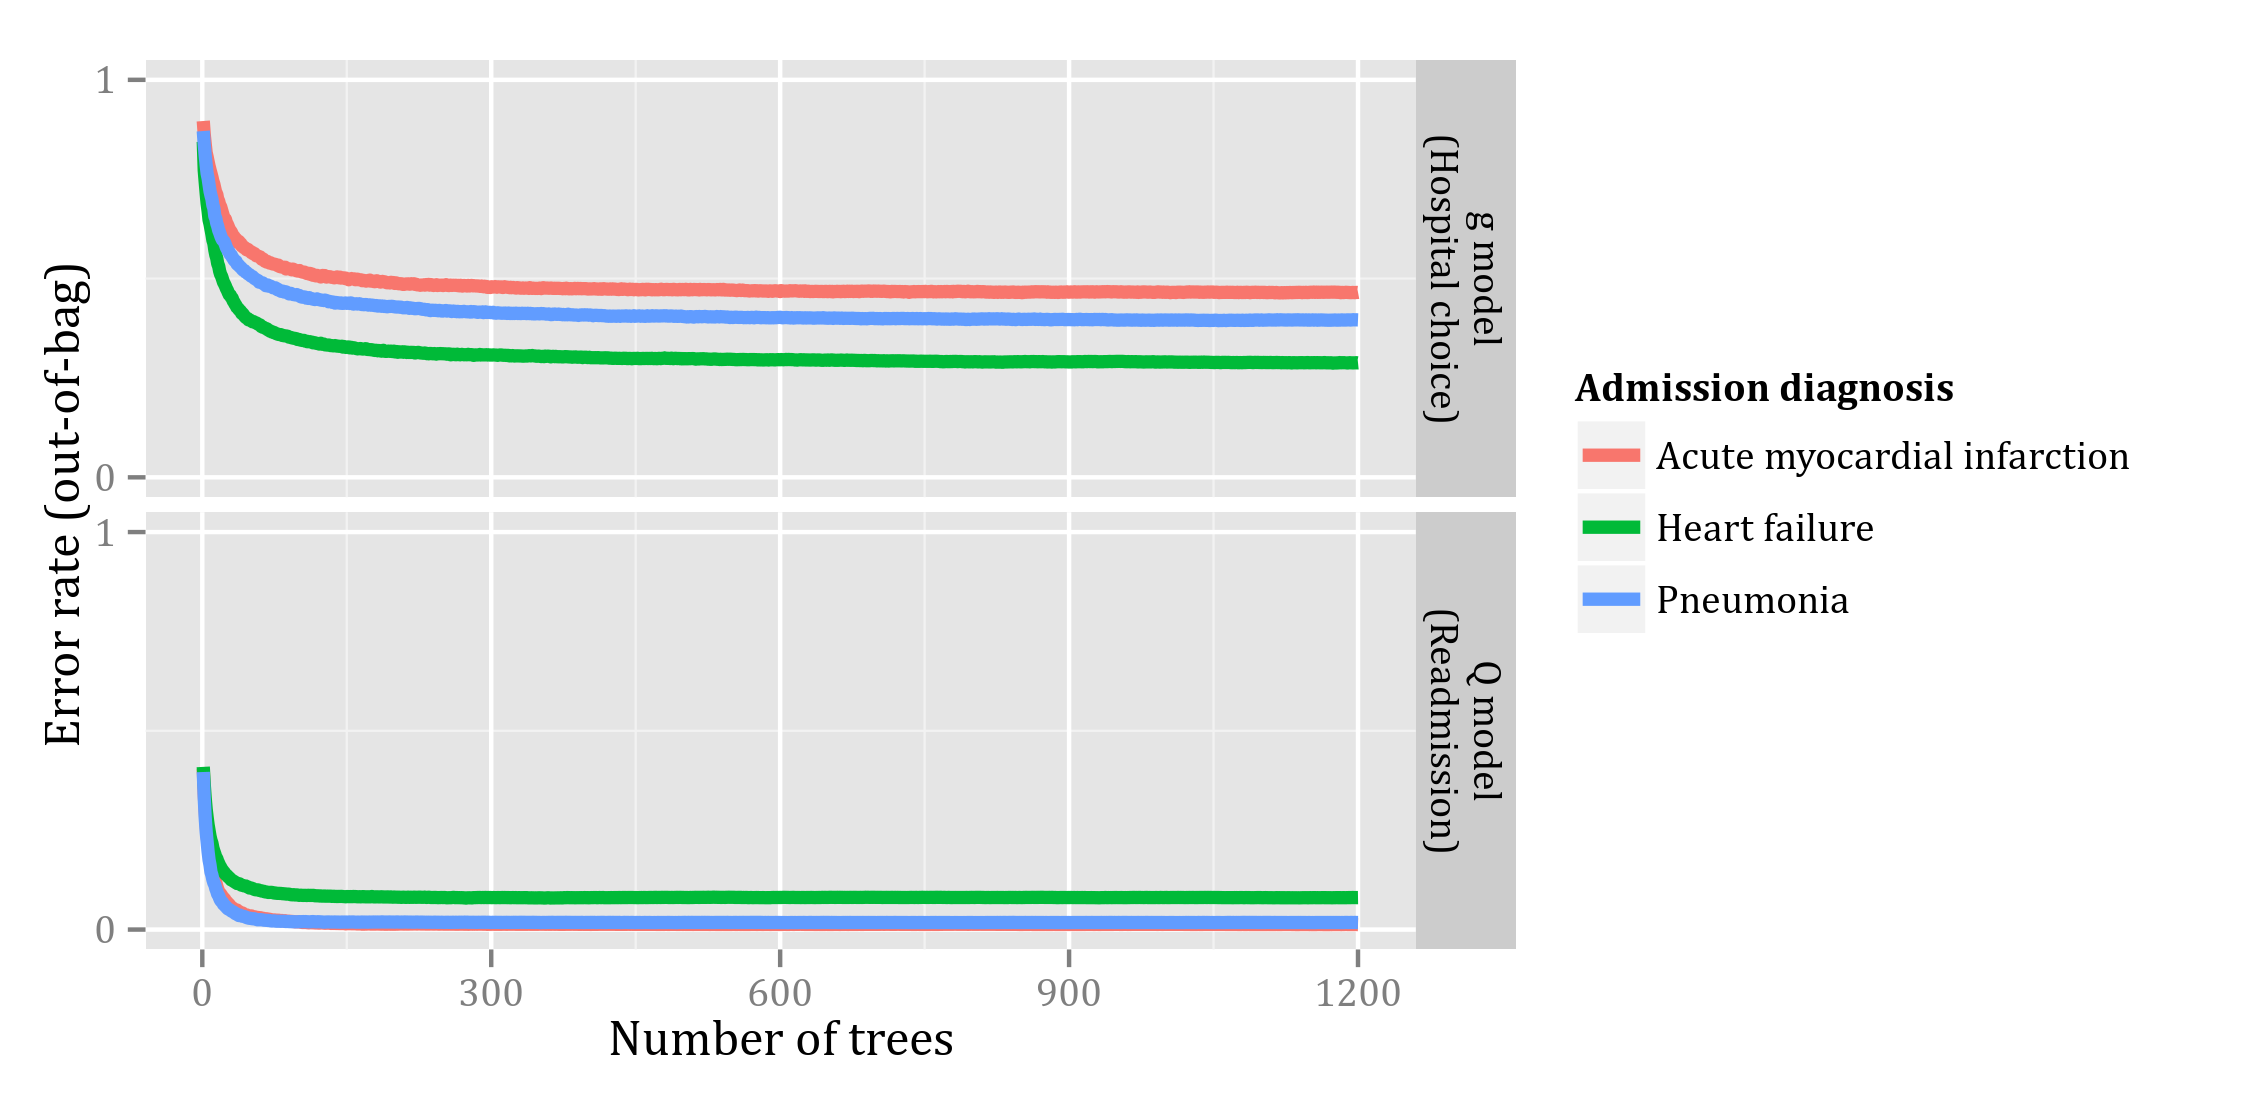
\includegraphics{../figures/error_rate_g_and_Q.png}
    \caption[Error rate for random forest model of hospital choice.]
      {Error rate for both random forest models of hospital choice ($g$) and readmission ($Q$) as a function of the number of trees grown. For each admission, only out-of-bag trees were used to predict the given outcome.}
    \label{fig:error_rate_for_g_and_Q}
\end{figure}


% Distribution of g
\begin{figure}[H]
    \includegraphics{../figures/dist_g_zoomed.png}
    \caption[Histogram of the probability of exposure ($g$), restricted to the range of (0,0.05). The bin width is 0.005. The dotted red lines indicate the two values of $\delta$ used in Tables 1, 2, and 3.]
      {Histogram of the probability of exposure ($g$), restricted to the range of (0,0.05). The bin width is 0.005. The dotted red lines indicate the two values of $\delta$ used in Tables 1, 2, and 3.}
    \label{fig:dist_g_zoomed}
\end{figure}

% A list of ICD9 codes used to select the cohort.
%latex.default(icd.codes, file = "", caption.loc = "bottom", label = "icd_codes",     longtable = TRUE, rowname = NULL)%
\setlongtables\begin{longtable}{ll}\hline\hline
\multicolumn{1}{c}{ICD9}&\multicolumn{1}{c}{Description}\tabularnewline
\hline
\endhead
\hline
\endfoot
100&Primary tuberculous infection, primary tuberculous complex\tabularnewline
101&Tuberculous pleurisy in primary progressive tuberculosis\tabularnewline
108&Other primary progressive tuberculosis\tabularnewline
109&Primary tuberculous infection, unspecified\tabularnewline
110&Tuberculosis of lung, infiltrative\tabularnewline
111&Tuberculosis of lung, nodular\tabularnewline
112&Tuberculosis of lung with cavitation\tabularnewline
113&Tuberculosis of bronchus\tabularnewline
114&Tuberculous fibrosis of lung\tabularnewline
115&Tuberculous bronchiectasis\tabularnewline
116&Tuberculous pneumonia (any form)\tabularnewline
117&Tuberculous pneumothorax\tabularnewline
118&Other pulmonary tuberculosis\tabularnewline
119&Pulmonary tuberculosis, unspecified\tabularnewline
203&Plague primary pneumonic\tabularnewline
204&Plague secondary pneumonic\tabularnewline
205&Plague pneumonic, unspecified\tabularnewline
219&Tularaemia\tabularnewline
221&Pulmonary anthrax\tabularnewline
249&Glanders\tabularnewline
259&Melioidosis\tabularnewline
320&Faucial diphtheria\tabularnewline
321&Nasopharyngeal diphtheria\tabularnewline
322&Anterior nasal diphtheria\tabularnewline
323&Laryngeal diphtheria\tabularnewline
329&Diphtheria, unspecified\tabularnewline
330&Whooping cough, bordetella pertussis (B.pertussis)\tabularnewline
331&Whooping cough, bordetella parapertussis (B.parapertussis)\tabularnewline
338&Whooping cough, other specified organism\tabularnewline
339&Whooping cough, unspecified organism\tabularnewline
340&Streptococcal sore throat\tabularnewline
529&Chickenpox\tabularnewline
&Chickenpox (varicella), uncomplicated\tabularnewline
551&Measles, postmeasles pneumonia\tabularnewline
739&Ornithosis\tabularnewline
741&Specific diseases due to coxsackie virus, epidemic pleurodynia\tabularnewline
790&Adenovirus\tabularnewline
793&Rhinovirus\tabularnewline
798&Other viral infection\tabularnewline
799&Viremia, unspecified\tabularnewline
\newpage
&Unspecified viral infection\tabularnewline
830&Rickettsioses, Q-fever\tabularnewline
1124&Candidiasis, of lung\tabularnewline
1149&Coccidioidomycosis\tabularnewline
1150&Infection by histoplasma capsulatum\tabularnewline
1151&Infection by histoplasma duboisii\tabularnewline
1159&Histoplasmosis, unspecified\tabularnewline
1309&Toxoplasmosis\tabularnewline
1363&Pneumocystosis\tabularnewline
3820&Suppurative and unspecified otitis media, acute suppurative otitis media\tabularnewline
3824&Unspecified suppurative otitis media\tabularnewline
3829&Unspecified otitis media\tabularnewline
4609&Acute nasopharyngitis (common cold), acute nasopharyngitis (common cold)\tabularnewline
4618&Acute sinusitis, other\tabularnewline
4619&Acute sinusitis, unspecified\tabularnewline
4629&Acute pharyngitis, acute pharyngitis\tabularnewline
4639&Acute tonsillitis, acute tonsillitis\tabularnewline
4640&Acute laryngitis\tabularnewline
4641&Acute tracheitis\tabularnewline
4642&Acute laryngotracheitis\tabularnewline
4643&Acute epiglottitis\tabularnewline
4644&Acute laryngitis and tracheitis, croup\tabularnewline
4650&Acute laryngopharyngitis\tabularnewline
4658&Other multiple sites\tabularnewline
4659&Acute upper respiratory infections, unspecified site\tabularnewline
&URTI, unspecified\tabularnewline
4660&Acute bronchitis\tabularnewline
4661&Acute bronchiolitis\tabularnewline
4789&Other and unspecified diseases of upper respiratory tract\tabularnewline
4800&Viral pneumonia, pneumonia due to adenovirus\tabularnewline
4801&Viral pneumonia, pneumonia due to respiratory syncytial virus\tabularnewline
4802&Viral pneumonia, pneumonia due to parainfluenza virus\tabularnewline
4808&Viral pneumonia, pneumonia due to other virus, not elsewhere classified\tabularnewline
4809&Viral pneumonia, viral pneumonia, unspecified\tabularnewline
4819&Pneumococcal pneumonia\tabularnewline
4820&Other bacterial pneumonia, pneumonia due to klebsiella pneumoniae\tabularnewline
4821&Other bacterial pneumonia, pneumonia due to pseudomonas\tabularnewline
4822&Pneumonia due to haemophilus influenzae (h.influenzae)\tabularnewline
4823&Other bacterial pneumonia, pneumonia due to streptococcus\tabularnewline
4824&Other bacterial pneumonia, pneumonia due to staphylococcus\tabularnewline
\newpage
4828&Other bacterial pneumonia, pneumonia due to other specified bacteria\tabularnewline
4829&Other bacterial pneumonia, bacterial pneumonia, unspecified\tabularnewline
4839&Pneumonia due to other specified organism\tabularnewline
4841&Cytomegalic inclusion disease\tabularnewline
4843&Pneumonia in infectious diseases classified elsewhere, whooping cough\tabularnewline
4845&Pneumonia in infectious diseases classified elsewhere, anthrax\tabularnewline
4846&Pneumonia in infectious diseases classified elsewhere, aspergillosis\tabularnewline
4847&Pneumonia in other systemic mycoses\tabularnewline
4848&Pneumonia in other infectious diseases\tabularnewline
4859&Bronchopneumonia, organism unspecified\tabularnewline
4869&Pneumonia, organism unspecified\tabularnewline
&Pneumonia, unspecified\tabularnewline
4870&Influenza, with pneumonia\tabularnewline
4871&Influenza (flu) NOS\tabularnewline
&Influenza, with other respiratory manifestations\tabularnewline
4878&Influenza, with other manifestations\tabularnewline
4909&Bronchitis, not specified as acute or chronic\tabularnewline
4910&Simple chronic bronchitis\tabularnewline
4911&Mucopurulent chronic bronchitis\tabularnewline
4918&Other chronic bronchitis\tabularnewline
4919&Chronic bronchitis, unspecified\tabularnewline
5070&Pneumonitis due to solids and liquids, due to inhalation of food or vomit\tabularnewline
5071&Due to inhalation of oils and essences\tabularnewline
5078&Pneumonitis due to solids and liquids, other\tabularnewline
5110&Pleurisy, without mention of effusion or current tuberculosis\tabularnewline
5111&With effusion, with mention of a bacterial cause other than tuberculosis\tabularnewline
5118&Pleurisy, other specified forms of effusion, except tuberculosis\tabularnewline
5119&Pleurisy, unspecified pleural effusion\tabularnewline
5130&Abscess of lung\tabularnewline
5131&Abscess of mediastinum\tabularnewline
5180&Other diseases of lung, pulmonary collapse\tabularnewline
5184&Other diseases of lung, acute oedema of lung, unspecified\tabularnewline
5188&Other diseases of lung, other diseases of lung, not elsewhere classified\tabularnewline
5192&Other diseases of respiratory system, mediastinitis\tabularnewline
7806&Chills\tabularnewline
&General symptoms, pyrexia of unknown origin\tabularnewline
&General symptoms: fever, not otherwise specified\tabularnewline
&Hyperthermia\tabularnewline
7841&Symptoms involving head and neck, throat pain\tabularnewline
7860&Dyspnoea and respiratory abnormalities\tabularnewline
\newpage
&Shortness of breath\tabularnewline
7861&Symptoms involving respiratory system and other chest symptoms, stridor\tabularnewline
7862&Symptoms involving respiratory system and other chest symptoms, cough\tabularnewline
7865&Symptoms involving respiratory system and other chest symptoms, chest pain\tabularnewline
&Pleurodynia\tabularnewline
7953&Nonspecific positive culture findings\tabularnewline
V018&Other communicable diseases\tabularnewline
\hline
\end{longtable}



\end{document}
